\iffalse
\documentclass[12pt]{article}
\usepackage{graphicx}
\usepackage[none]{hyphenat}
\usepackage{graphicx}
\usepackage{listings}
\usepackage[english]{babel}
\usepackage{graphicx}
\usepackage{caption} 
\usepackage{booktabs}
\usepackage{array}
\usepackage{amssymb} % for \because
\usepackage{amsmath}   % for having text in math mode
\usepackage{extarrows} % for Row operations arrows
\usepackage{listings}
\lstset{
  frame=single,
  breaklines=true
}
\usepackage{hyperref}
  
%Following 2 lines were added to remove the blank page at the beginning
\usepackage{atbegshi}% http://ctan.org/pkg/atbegshi
\AtBeginDocument{\AtBeginShipoutNext{\AtBeginShipoutDiscard}}


%New macro definitions
\newcommand{\mydet}[1]{\ensuremath{\begin{vmatrix}#1\end{vmatrix}}}
\providecommand{\brak}[1]{\ensuremath{\left(#1\right)}}
\providecommand{\norm}[1]{\left\lVert#1\right\rVert}
\providecommand{\abs}[1]{\left\vert#1\right\vert}
\newcommand{\solution}{\noindent \textbf{Solution: }}
\newcommand{\myvec}[1]{\ensuremath{\begin{pmatrix}#1\end{pmatrix}}}
\let\vec\mathbf


\begin{document}

\begin{center}
\title{\textbf{Conic Sections - Parbola}}
\date{\vspace{-5ex}} %Not to print date automatically
\maketitle
\end{center}
\setcounter{page}{1}

\section{11$^{th}$ Maths - Chapter 11}
This is Problem-1 from Exercise 11.2
\begin{enumerate}
\solution 
\fi
The given equation of the parabola can be rearranged as
\begin{align}
    \label{eq:chapters/11/11/2/1/parabolaEq1}
    y^2-12x = 0
\end{align}
The above equation can be equated to the generic equation of conic sections
\begin{align}
	\label{eq:chapters/11/11/2/1/parabolaEq2}
	g\brak{\vec{x}} = \vec{x}^T\vec{V}\vec{x} + 2\vec{u}^T\vec{x} + f = 0 
\end{align}
Comparing coefficients of \eqref{eq:chapters/11/11/2/1/parabolaEq1} and \eqref{eq:chapters/11/11/2/1/parabolaEq2},
\begin{align}
	\label{eq:chapters/11/11/2/1/eqV}
	\vec{V} &= \myvec{ 0 & 0 \\ 0 & 1} \\
	\label{eq:chapters/11/11/2/1/eqU}
	\vec{u} &= -\myvec{6 \\ 0} \\
	\label{eq:chapters/11/11/2/1/eqF}
	f &= 0 
\end{align}
\begin{enumerate}
\item  
From \eqref{eq:chapters/11/11/2/1/eqV}, since $\vec{V}$ is already diagonalized, the Eigen values $\lambda_1$ and $\lambda_2$ are given as 
\begin{align}
	\label{eq:chapters/11/11/2/1/eqEigen1}
	\lambda_1 &= 0 \\
	\label{eq:chapters/11/11/2/1/eqEigen2}
	\lambda_2 &= 1 
\end{align}
and the eigenvector matrix
\begin{align}
	\vec{P} = \vec{I}.
\end{align}
\iffalse
The Eigen vector $\vec{p_1}$ corresponding to Eigen value $\lambda_1$ is computed as shown below
\begin{align}
	\vec{V} &= \myvec{ 0 & 0 \\ 0 & 1} \\
	\label{eq:chapters/11/11/2/1/eqLambda1}
	\vec{V}-\lambda_1\vec{I} &= \myvec{ 0 - \lambda_1 & 0 \\ 0 & 1-\lambda_1} 
\end{align}
Substituting value of $\lambda_1$ from \eqref{eq:chapters/11/11/2/1/eqEigen1} in \eqref{eq:chapters/11/11/2/1/eqLambda1}
\begin{align}
	\eqref{eq:chapters/11/11/2/1/eqLambda1} \implies  \myvec{  0 & 0 \\ 0 & 1}  \\
	\myvec{  0 & 0 \\ 0 & 1}\myvec{x_1 \\ x_2} &= \myvec{0 \\0} 
\end{align}
$x_1$ is free variable and $x_2 = 0$. \\
\fi
\begin{align}
	\therefore 
	%\vec{p_1} &= \myvec{1 \\ 0} \\
	\vec{n} &= \sqrt{\lambda_2}\vec{p_1} \\
%	&= \sqrt{1}\myvec{1 \\ 0} \\
	\label{eq:chapters/11/11/2/1/eqN}
	&= \myvec{1 \\ 0} 
\end{align}
Since
\begin{align}
	\label{eq:chapters/11/11/2/1/eqC}
	c = \frac{\norm{\vec{u}^2}-\lambda_2f}{2\vec{u}^\top\vec{n}},
\end{align}
Substituting values of $\vec{u}, \vec{n}, \lambda_2 \text{ and } f$ in \eqref{eq:chapters/11/11/2/1/eqC}
\begin{align}
	c &= \frac{6^2-1\brak{0}}{-2 \myvec{6 & 0}\myvec{1 \\ 0}} = -3 \\
\end{align}
The focus $\vec{F}$ of parabola is expressed as
\begin{align}
	\vec{F} &= \frac{ce^2\vec{n}-\vec{u}}{\lambda_2} \\
	&= \frac{-3\brak{1}^2\myvec{1 \\0} + \myvec{6 \\ 0}}{1} \\
	&= \myvec{3 \\ 0}
\end{align}
\item The directrix is given by
\begin{align}
	\vec{n}^\top\vec{x} &= c \\
	\label{eq:chapters/11/11/2/1/eqDir}
\implies	\myvec{1 & 0}\vec{x} &= -3
\end{align}

\item The equation for the axis of parabola passing through $\vec{F}$ and orthogonal to the directrix is given as  
\begin{align}
	\label{eq:chapters/11/11/2/1/eqAxis}
	\vec{m}^\top\brak{\vec{x}-\vec{F}} &= 0
\end{align}
where $\vec{m}$ is the normal vector to the axis and also the slope of the directrix.
\begin{align}
	\because \vec{n} = \myvec{1 \\ 0 }, \vec{m} &= \myvec{0 \\ 1} \\
	\eqref{eq:chapters/11/11/2/1/eqAxis} \implies \myvec{0 & 1}\myvec{\vec{x} - \myvec{3 \\ 0}} &= 0\\
	\text{or, }	\myvec{0 & 1}\vec{x} &= 0 
\end{align}
\item The latus rectum of a parabola is given by 
\begin{align}
	l &= \frac{\eta}{\lambda_2}  
	 = \frac{2\vec{u}^\top\vec{p_1}}{\lambda_2} \\
	 &= \frac{2\myvec{6 & 0}\myvec{1 \\ 0}}{1} \\
	 &= 12 \text{ units }
\end{align}
The relevant diagram is shown in Fig. \ref{fig:11/11/2/1Fig1}
\begin{figure}[!h]
	\begin{center}
		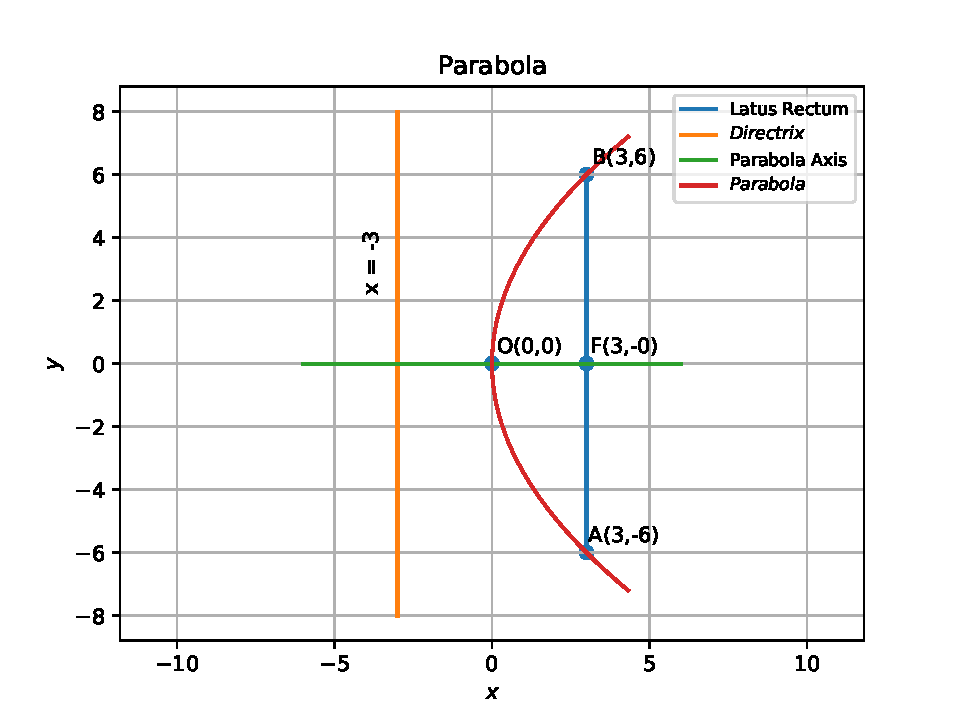
\includegraphics[width=\columnwidth]{chapters/11/11/2/1/figs/problem1.pdf}
	\end{center}
\caption{}
\label{fig:11/11/2/1Fig1}
\end{figure}
\end{enumerate}
